\chapter{Data}
\label{cha:data}

\section{Data acquisition}
\label{sec:data-acquisition}

The data was acquired at the \acrfull{sas} laboratory at Linköping University. The experiment --- as shown on Figure~\ref{fig:experimental-setup} --- consisted of exposing different gas combinations to two \acrshort{sicfet} sensors under a particular frequency cycle and recording its response, measured in \acrfull{ma}. The is then used to extract secondary features, namely average and slope values from certain regions of the frequency cycle.

\begin{figure}[!htb]
	\centering
	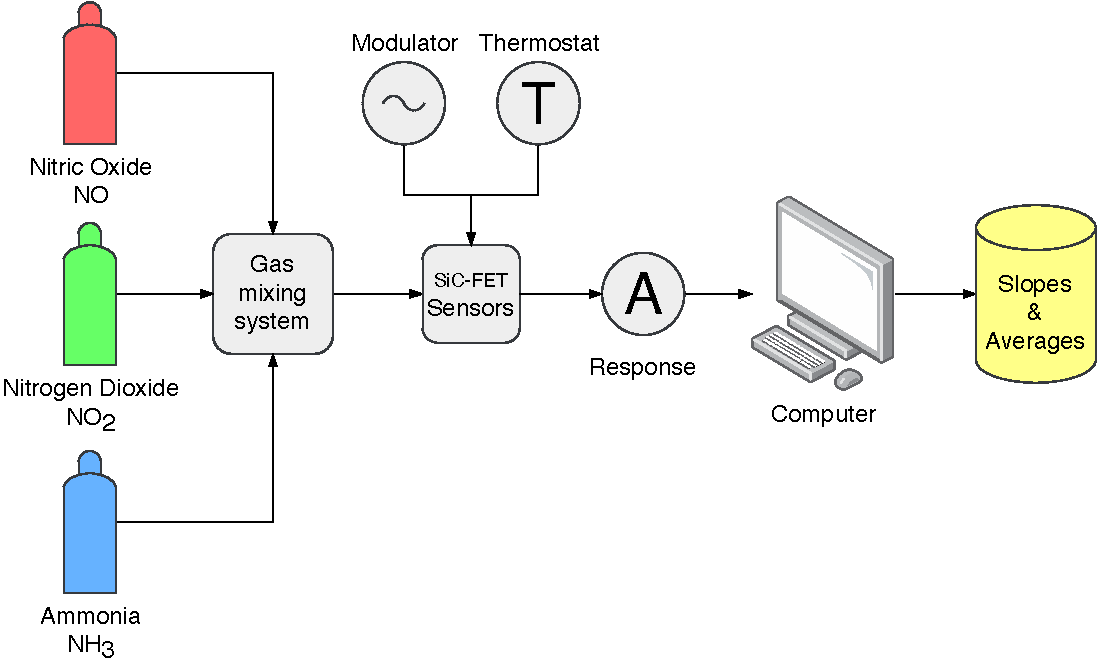
\includegraphics[width=0.8\textwidth]{../figures/experimental-setup.pdf}
	\caption{Schema of the data acquisition process.}
	\label{fig:experimental-setup}
\end{figure}

In more detail, \ch{NO}, \ch{NO2} and \ch{NH3} had five possible concentration values each: 5, 10, 20, 40, and 80 \acrfull{ppm}. The experiment was designed to encompass all possible combinations of these gases, amounting to 125 different gas mixtures. Each feature was submitted to the same frequency cycle four times. The cycle consists of 16 unique frequencies: 0.05, 0.1, 0.25, 0.5, 1, 2, 5, 10, 25, 50, 100, 200, 500, 1000, 2500 and 5000 \acrfull{hertz}. A typical raw sensor response for frequency modulation experiments is shown on Figure~\ref{fig:raw}.

\begin{figure}[!htb]
	\centering
	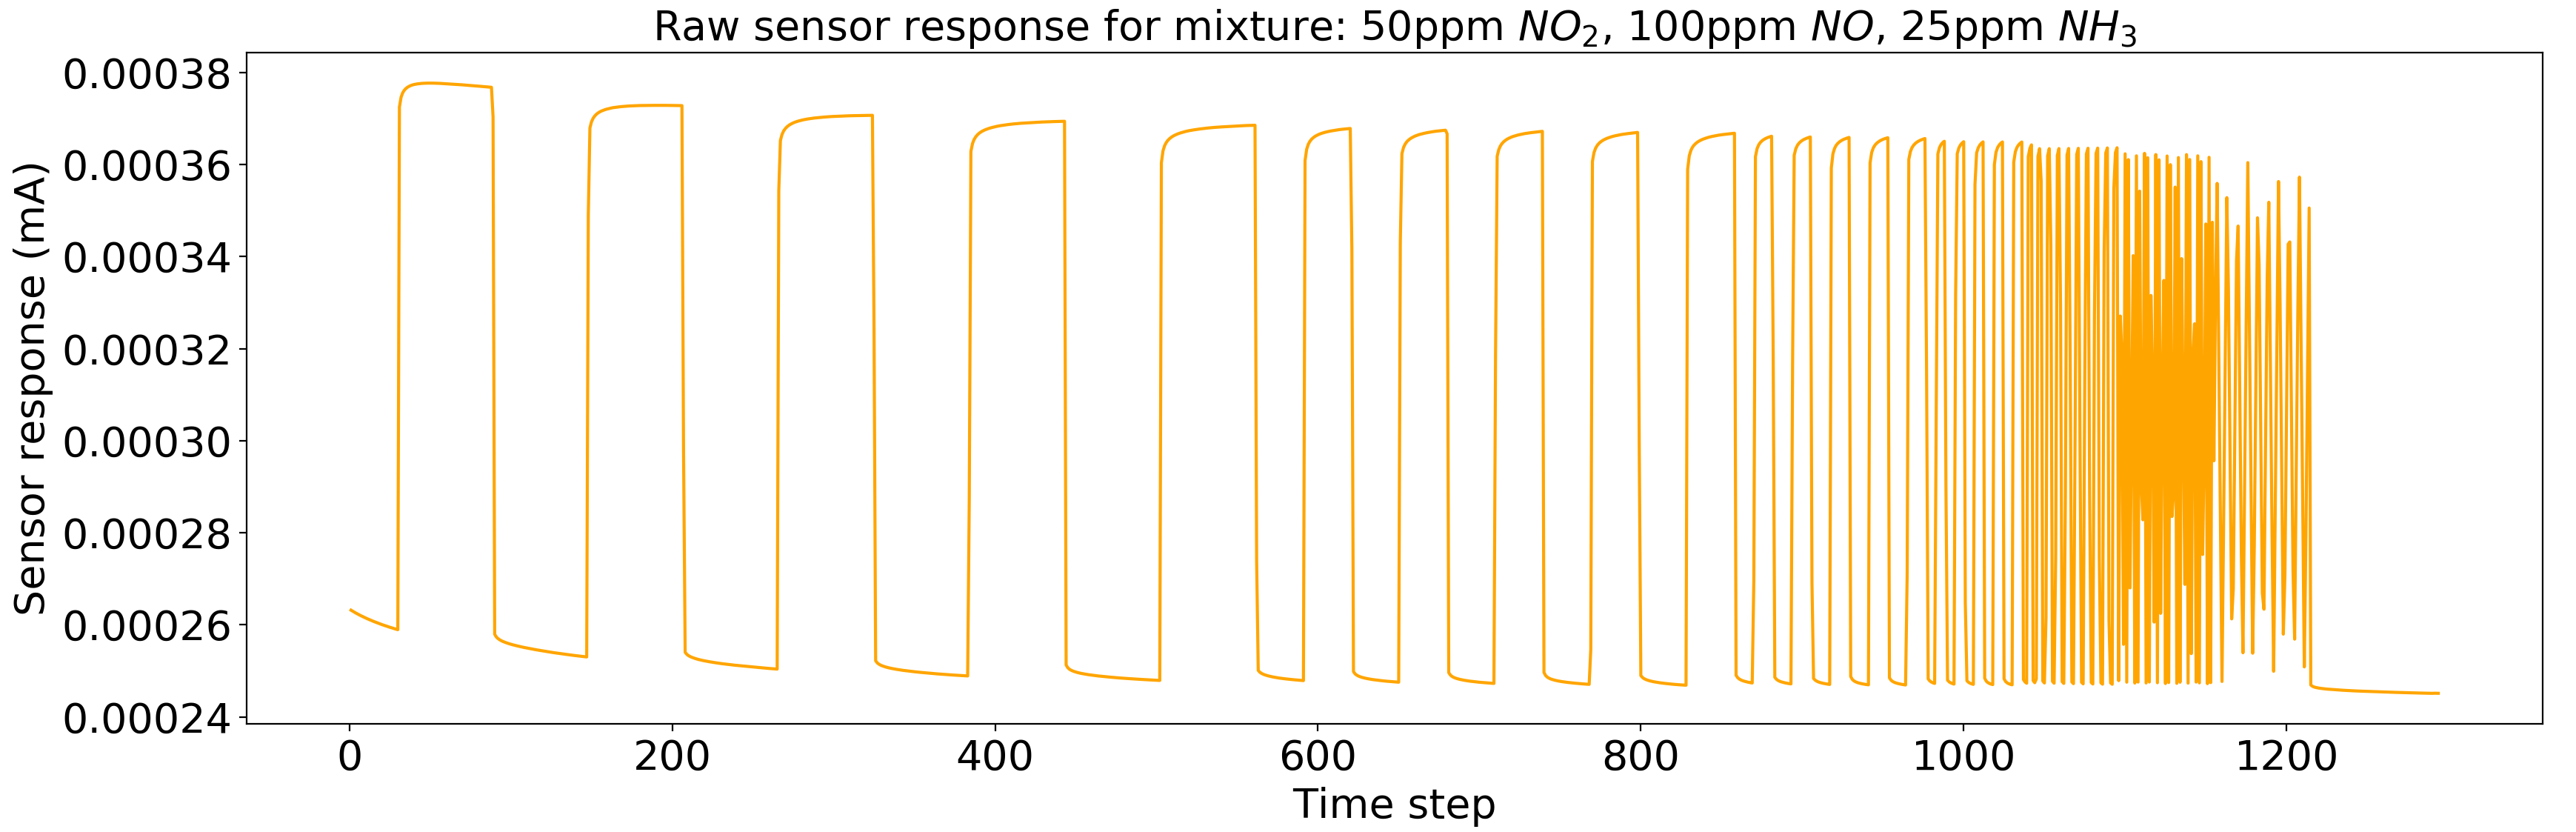
\includegraphics[width=1\textwidth]{../figures/raw-response.png}
	\caption{An example of row sensor response}
	\label{fig:raw}
\end{figure}

Throughout one cycle, several slope and average features were extracted. The sample rate for feature extraction was set at 4 \acrshort{hertz}, i.e. in a cycle of 60 seconds, a total of $60 \text{s} \times 4 \frac{1}{\text{s}} = 240$ pairs of slopes and averages are recorded, which totals to 480 features per cycle. In other words, during one experiment --  4 cycles of 60 seconds -- a total of $480 \times 4 = 1920$ features are extracted. 

One way to visualize this process is shown in Figures~\ref{fig:feat-window}. Note that the y-axis is in log-scale due to the different orders of magnitude of frequencies. Moreover, Figure~\ref{fig:features} gives more insight into feature measurement and Table~\ref{tab:measurements} summarizes the data acquisition details.

\begin{figure}[!htb]
	\centering
	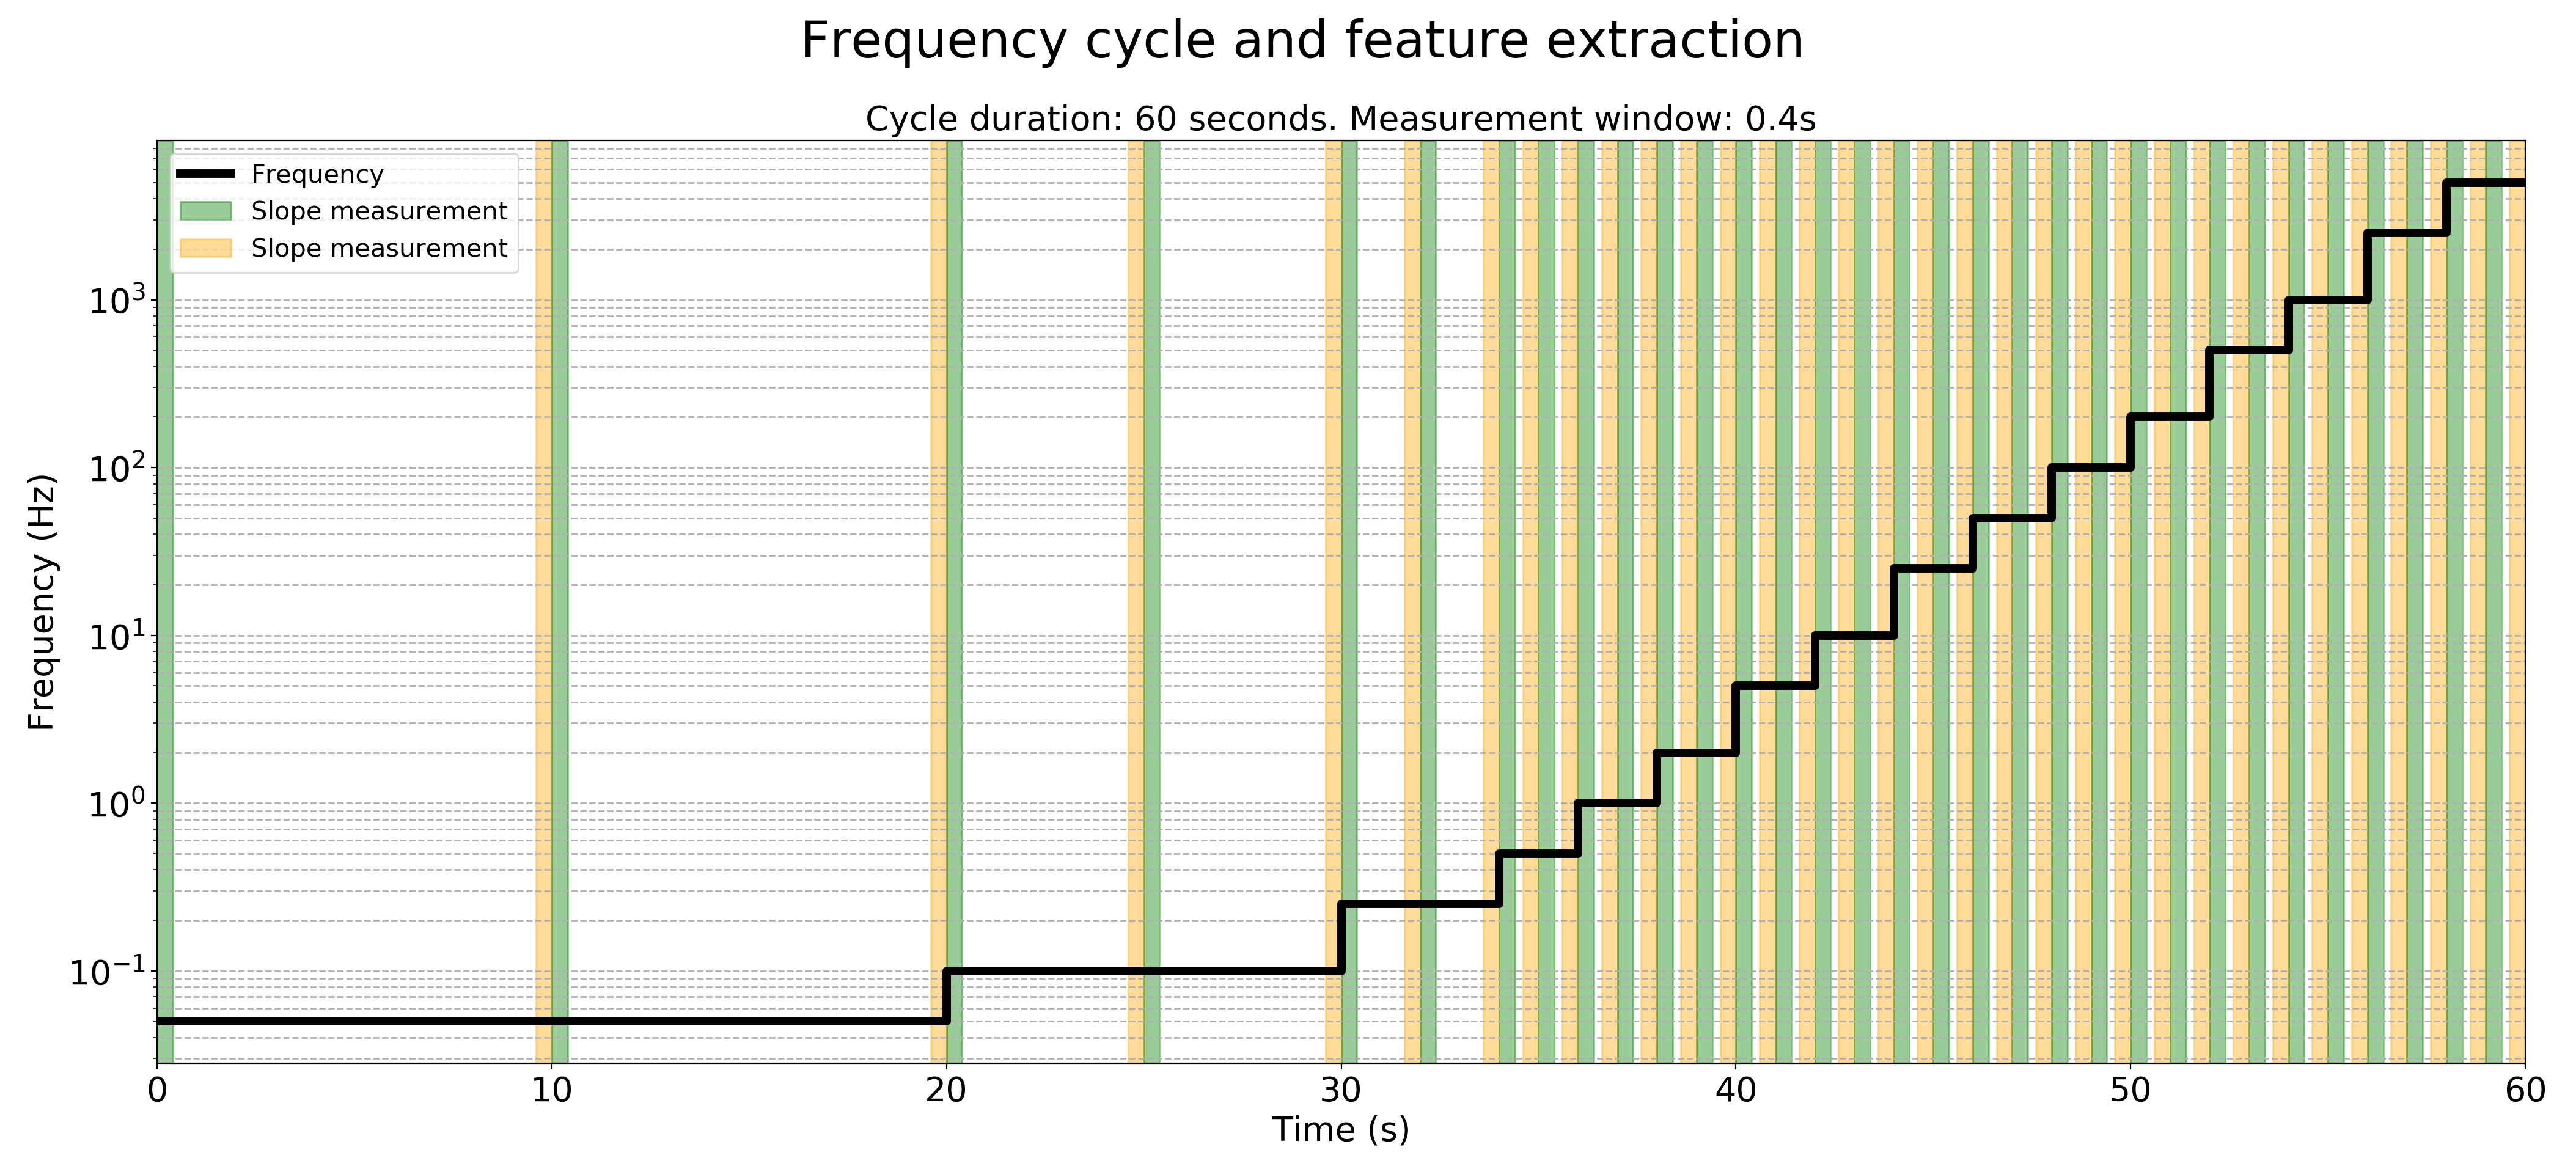
\includegraphics[width=1\textwidth]{../figures/measurement-windows.png}
	
	\caption{Feature measurements times per cycle.}
	\label{fig:feat-window}
\end{figure} 

\begin{figure}[h]
	\centering
	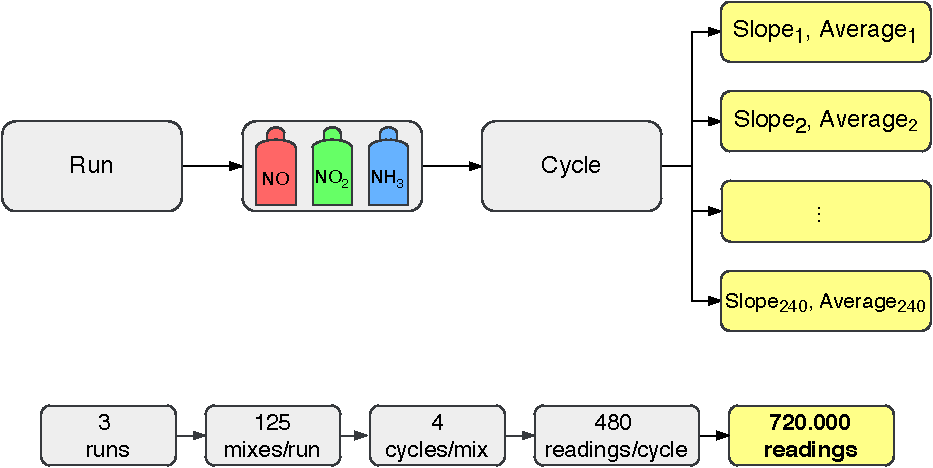
\includegraphics[width=1\textwidth]{../figures/features.pdf}
	\caption{A visualization of the feature measurement process.}
	\label{fig:features}
\end{figure}

\begin{table}[h]
	\centering
	\caption{Data acquisition details}
	\label{tab:measurements}
	\begin{tabular}{|c|c|}
		\hline
		\textbf{Parameter} & \textbf{Value} \\
		\hline
		Factors (gases) & 3 \\
		\hline
		Levels (concentrations) & 5 \\
		\hline
		Frequencies & 16 \\
		\hline
		Features per cycle & 480 \\
		\hline
		Number of cycles & 4 \\
		\hline
		Data points per mixture & 1920\\
		\hline
		Number of mixtures & 125 \\
		\hline
		Features per experiment & 240.000 \\
		\hline
		Number of experiments & 3 \\
		\hline
		Total features & 720.000 \\
		\hline
	\end{tabular}
\end{table}

For specific timestamps and measurement durations, the reader is referred to Appendix~\ref{app:A}.

\section{Raw data}
\label{sec:raw-data}

The experiments were run between 26th and 29th March, 2021. The experiment data was exported as an excel file containing twelve columns, as specified in Table~\ref{tab:raw-cols}


\begin{table}[h]
	\centering
	\caption{Raw data column details}
	\label{tab:raw-cols}
	
	\resizebox{\textwidth}{!}{%
		\begin{tabular}{|c|c|c|}
		\hline
		\textbf{Name} & \textbf{Description} & \textbf{Unit} \\
		\hline
		Exposure nr & A particular mix of NO, NO$_2$ and NH$_3$. Ranges from 1 to 375  & -\\
		\hline
		Cycle nr & The cycle number. Ranges from 1 to 4. & - \\
		\hline
		Sample nr & Extracted feature index. Ranges from 1 to 240 & - \\
		\hline
		NO & Nitric Oxide concentration & \acrshort{ppm} \\
		\hline
		NO2 & Nitrogen Dioxide concentration &\acrshort{ppm} \\
		\hline
		NH3 & Ammonia concentration &\acrshort{ppm} \\
		\hline
		Freq & Frequency & \acrshort{hertz}\\
		\hline
		Slope sensor 1 & Slope & $\mu$A/s \\
		\hline
		Slope sensor 2 & Slope & $\mu$A/s\\
		\hline
		Average sensor 1 & Average & $\mu$A \\
		\hline
		Average sensor 2& Average & $\mu$A\\
		\hline
		Sensor temperature & Temperature & degrees Celsius ($^{\circ}$C) \\
		\hline
	\end{tabular}}
\end{table}

\begin{table}
	\centering
	\caption{Sample of raw data.}
	\label{tab:raw-sample}
	\resizebox{\textwidth}{!}{%
		\begin{tabular}{p{1.5cm}p{1.3cm}p{0.8cm}p{1.3cm}p{0.8cm}p{0.8cm}p{1.8cm}p{1.8cm}p{1.8cm}p{1.8cm}p{1.8cm}p{1.8cm}p{1.8cm}}
		\toprule[0.5mm]
		Index & Exposure\newline nr &  Cycle\newline  nr &  Sample\newline  nr &  NO\newline  [ppm] &  NO2\newline  [ppm] &  NH3\newline  [ppm] &  Freq\newline  [Hz] &  Slope\newline  sensor 1\newline [uA/s] &  Slope\newline  sensor 2\newline [uA/s] &  Average\newline  sensor 1\newline [uA/s] &  Average\newline  sensor 2\newline [uA/s] &  Sensor\newline  temperature \newline[C] \\
		\midrule[0.5mm]
		0 &            1 &         1 &          1 &        10 &          5 &         20 &       0.05 &             -18.855169 &             -22.588416 &                32.926184 &                27.961554 &              274.994683 \\
		1 &            1 &         1 &          2 &        10 &          5 &         20 &       0.05 &             -28.289268 &             -28.185027 &                25.853867 &                20.915297 &              274.980487 \\
		2 &            1 &         1 &          3 &        10 &          5 &         20 &       0.05 &              -0.390916 &              -0.482129 &                25.756138 &                20.794765 &              274.985895 \\
		3 &            1 &         1 &          4 &        10 &          5 &         20 &       0.05 &              -0.234549 &              -0.156366 &                25.697501 &                20.755673 &              275.020372 \\
		4 &            1 &         1 &          5 &        10 &          5 &         20 &       0.05 &              -0.143336 &              -0.247580 &                25.661667 &                20.693778 &              275.014964 \\
		
		\bottomrule
		&&&&&&&&&&&&\\
		&&&&&&&\sbox0{\dots}\makebox[\wd0]{\vdots}&&&&&\\
		&&&&&&&&&&&&\\
		\toprule
		
		100000 &          105 &         1 &        161 &         5 &          5 &         40 &        5.0 &             -38.366212 &             -48.495271 &                30.241896 &                24.821197 &              275.021724 \\
		100001 &          105 &         1 &        162 &         5 &          5 &         40 &        5.0 &               6.619507 &               8.521964 &                31.896773 &                26.951688 &              274.999415 \\
		100002 &          105 &         1 &        163 &         5 &          5 &         40 &        5.0 &              -1.941549 &               6.580416 &                31.411386 &                28.596792 &              275.011584 \\
		100003 &          105 &         1 &        164 &         5 &          5 &         40 &        5.0 &              27.401023 &              22.012900 &                38.261641 &                34.100017 &              275.009894 \\
		100004 &          105 &         1 &        165 &         5 &          5 &         40 &        5.0 &             -27.016623 &             -28.439121 &                31.507486 &                26.990236 &              275.014400 \\
		\bottomrule
		&&&&&&&&&&&&\\
		&&&&&&&\sbox0{\dots}\makebox[\wd0]{\vdots}&&&&&\\
		&&&&&&&&&&&&\\
		\toprule
		
		359995 &          375 &         4 &        236 &        20 &         80 &          5 &     5000.0 &              -0.136821 &              -0.158538 &                34.129879 &                30.345597 &              275.002007 \\
		359996 &          375 &         4 &        237 &        20 &         80 &          5 &     5000.0 &               0.010859 &               0.010859 &                34.132593 &                30.348312 &              274.986797 \\
		359997 &          375 &         4 &        238 &        20 &         80 &          5 &     5000.0 &              -0.043435 &               0.030405 &                34.121734 &                30.355913 &              274.979811 \\
		359998 &          375 &         4 &        239 &        20 &         80 &          5 &     5000.0 &              -0.117275 &              -0.026061 &                34.092416 &                30.349398 &              274.984543 \\
		359999 &          375 &         4 &        240 &        20 &         80 &          5 &     5000.0 &               0.073840 &               0.039092 &                34.110876 &                30.359171 &              274.998063 \\
		\bottomrule[0.5mm]
	\end{tabular}}
\end{table}

\newpage
\section{Pre-processing}
\label{sec:preprocessing}

The features (slopes and averages) from the same target (a particular exposure) in the raw data file  are spread across multiple rows, which is not suitable for analysis. Opposed to \acrshort{tco}, the experiments were conducted at constant temperature and therefore the temperature column is discarded. The data was, subsequently, modified to have the desired format: each row containing the predictors for one particular combination of gases. Additionally, the data from each sensor was split into  two datasets. 

The naming convention for the features is shown in Figure~\ref{fig:feat-naming}. First, the frequency in which the measurement was taken followed by the sensor number. After that, the feature name itself is followed by its index, i.e. where in the frequency cycle the measurement was made. This convention allows for easy identification of key information of the cycle and measurement.

\begin{figure}[h]
	\centering
	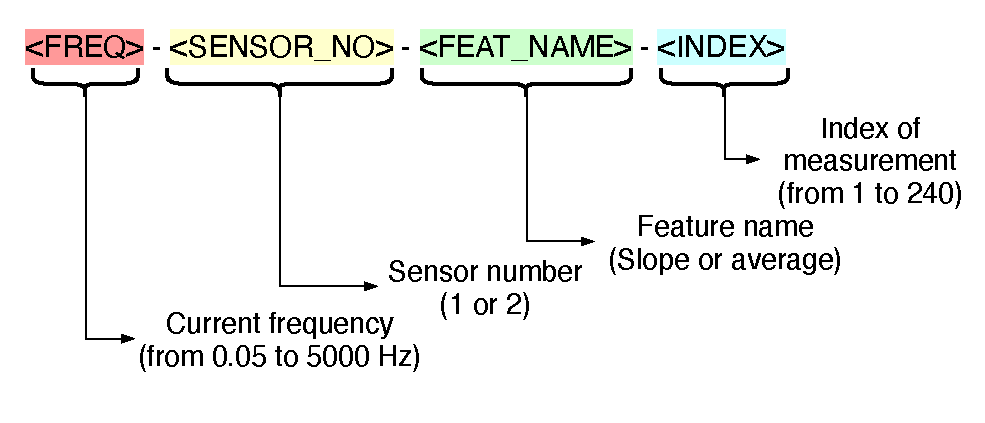
\includegraphics[width=1\textwidth]{../figures/feat-naming.pdf}
	\caption{Feature naming convention.}
	\label{fig:feat-naming}
\end{figure}

The pre-processing results in the format shown in Figure~\ref{fig:preprocessed-data}. Recalling that there are 125 possible mixtures of gases, it is important to note that there are repeated exposures in the data set and those are treated as individual observations. Since each unique gas mixture was exposed 4 times during a cycle, and the experiment was repeated 3 times. This yields a total of $4 \times 3 \times 125 = 1500$ exposures.

\begin{figure}[h]
	\centering
	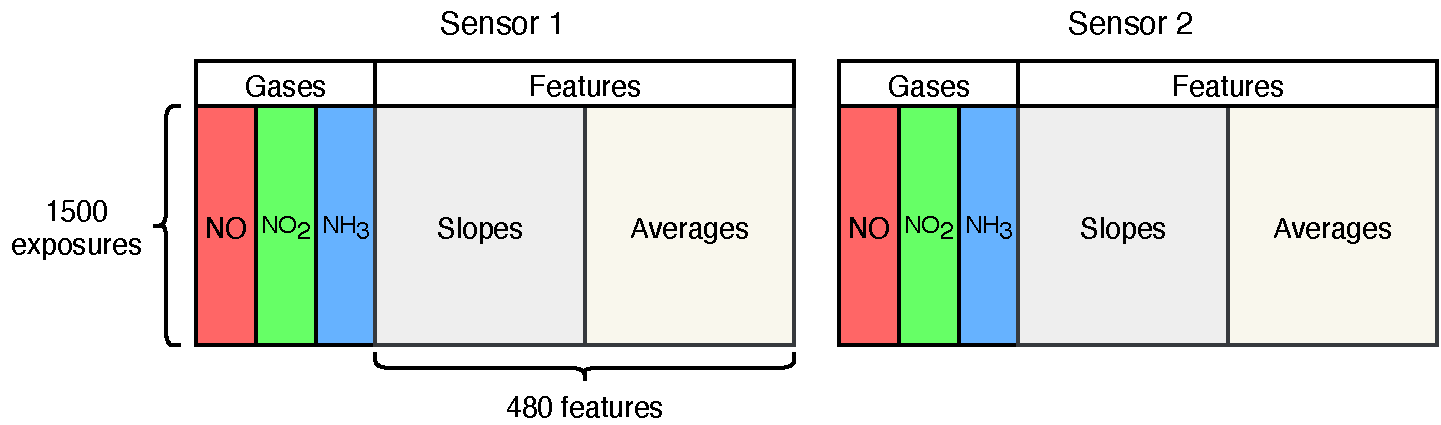
\includegraphics[width=1\textwidth]{../figures/preprocessed-data.pdf}
	\caption{Pre-processed data structure.}
	\label{fig:preprocessed-data}
\end{figure}

Finally, the majority of models proposed are scale variant, with the exception of \acrshort{ols}. The data, therefore, was centered and scaled to have unit variance and zero mean. A snippet of the final data set is shown in Table~\ref{tab:prepro-sample}


\begin{table}
	\centering
	\caption{Sample of pre-processed data.}
	\label{tab:prepro-sample}
	\resizebox{\textwidth}{!}{%
	\begin{tabular}{cp{1.3cm}p{0.8cm}p{0.8cm}p{0.8cm}p{1.8cm}p{1.8cm}p{0.3cm}p{1.6cm}p{1.6cm}p{1.6cm}p{1.6cm}p{0.3cm}p{1.6cm}p{1.6cm}}
		\toprule[0.5mm]
		Index &  exposure &    NO &   NO2 &   NH3 &  0.05-1-slope-0 &  0.05-1-slope-1 & $\dots$&  5000.0-1-slope-239 &  0.05-1-avg-0 &  0.05-1-avg-1 &  0.05-1-avg-2 & $\dots$&  5000.0-1-avg-238 &  5000.0-1-avg-239 \\
		\midrule[0.5mm]
		0 &       1.0 &  10.0 &   5.0 &  20.0 &        2.033884 &       -2.024181 &$\dots$&            1.256538 &      2.619349 &      1.757883 &      1.728610 & $\dots$&         2.276652 &          2.301890 \\
		1 &       1.0 &  10.0 &   5.0 &  20.0 &       -0.661288 &        0.869532 &$\dots$&           -0.846043 &      0.567699 &      2.477401 &      2.449619 & $\dots$&          2.522155 &          2.496103 \\
		2 &       1.0 &  10.0 &   5.0 &  20.0 &        0.232116 &        0.038766 &$\dots$&            1.546549 &      1.389922 &      2.716136 &      2.746701 & $\dots$&         2.637892 &          2.669321 \\
		3 &       1.0 &  10.0 &   5.0 &  20.0 &       -0.854716 &        1.071274 &$\dots$&            1.546549 &      0.592878 &      2.848766 &      2.866869 & $\dots$&         2.722064 &          2.753305 \\
		4 &       2.0 &  20.0 &  40.0 &  40.0 &        1.876790 &       -1.808299 &$\dots$&           -1.063551 &      2.963172 &      2.760346 &      2.746701 & $\dots$&         2.213523 &          2.182912 \\
		\bottomrule
		&&&&&&&&&&&&&&\\
		&&&&&&&\sbox0{\dots}\makebox[\wd0]{\vdots}&&&&&&&\\
		&&&&&&&&&&&&&&\\
		\toprule
		
		700 &     176.0 &  40.0 &  20.0 &  40.0 &        1.735014 &       -1.850717 & $\dots$&            -2.151093 &      1.590775 &      0.071822 &      0.072959 & $\dots$&          0.098694 &          0.046562 \\
		701 &     176.0 &  40.0 &  20.0 &  40.0 &       -0.466435 &        0.439147 & $\dots$&           -1.208557 &     -0.393152 &     -0.046993 &     -0.033022 &$\dots$&           0.084665 &          0.055310 \\
		702 &     176.0 &  40.0 &  20.0 &  40.0 &       -0.509181 &        0.495187 &  $\dots$&          -0.725205 &     -0.423540 &     -0.015217 &     -0.020505 & $\dots$&          0.078820 &          0.061143 \\
		703 &     176.0 &  40.0 &  20.0 &  40.0 &       -0.494932 &        0.467598 & $\dots$&           -2.296098 &     -0.409070 &     -0.031795 &     -0.043871 & $\dots$&          0.070052 &          0.014485 \\
		704 &     177.0 &  80.0 &  40.0 &  40.0 &        1.763512 &       -1.868305 &  $\dots$&           2.005733 &      1.608140 &      0.076796 &      0.059607 &$\dots$&           0.074144 &          0.122381 \\
		
		\bottomrule
		&&&&&&&&&&&&&&\\
		&&&&&&&\sbox0{\dots}\makebox[\wd0]{\vdots}&&&&&&&\\
		&&&&&&&&&&&&&&\\
		\toprule
		
		1495 &     374.0 &  80.0 &  80.0 &  40.0 &       -0.429032 &        0.485703 & $\dots$&          -0.725205 &     -1.122473 &     -1.365005 &     -1.369615 &$\dots$&         -1.476030 &         -1.490233 \\
		1496 &     375.0 &  20.0 &  80.0 &   5.0 &        1.083129 &       -1.205831 & $\dots$&          -1.426065 &      0.366557 &     -1.232375 &     -1.238876 & $\dots$&        -1.479537 &         -1.510646 \\
		1497 &     375.0 &  20.0 &  80.0 &   5.0 &       -0.635640 &        0.696067 & $\dots$&           0.507342 &     -1.303357 &     -1.373294 &     -1.352369 & $\dots$&        -1.461417 &         -1.445908 \\
		1498 &     375.0 &  20.0 &  80.0 &   5.0 &       -0.016883 &        0.086357 &  $\dots$&          0.120661 &     -0.768521 &     -1.329084 &     -1.358488 & $\dots$&        -1.481875 &         -1.475653 \\
		1499 &     375.0 &  20.0 &  80.0 &   5.0 &       -0.588619 &        0.638821 &  $\dots$ &          0.676515 &     -1.247789 &     -1.358926 &     -1.369615 & $\dots$&        -1.486551 &         -1.466904 \\
		\bottomrule[0.5mm]
	\end{tabular}}
\end{table}




